\documentclass[]{final_report}
\usepackage{graphicx}
\usepackage{hyperref}


%%%%%%%%%%%%%%%%%%%%%%
%%% Input project details
\def\studentname{Oraz Ospanov, Asset Malik, Andrey Yershov}
\def\projecttitle{Data-Driven Control for DC Motors}
\def\supervisorname{Do Duc Ton}

\begin{document}

\maketitle

\pdfbookmark[0]{Table of Contents}{toc}
\tableofcontents
\newpage

%%%%%%%%%%%%%%%%%%%%%%
%%% Your Abstract here

\begin{abstract}

\textbf{\textsl{Insert abstract here (see details later in these guidelines).}}

\end{abstract}
\newpage

%%%%%%%%%%%%%%%%%%%%%%
%%% Acknowledgments

\chapter*{Acknowledgments}

In your Acknowledgments section, give credit to all the people who helped you in your project.

%%%%%%%%%%%%%%%%%%%%%%
%%% Introduction

\chapter{Introduction}
\subsection{Model Based Control}

The modern control theory, also known as Model Based Control has been used both for linear and non-linear systems extensively since 1960. The Model Based Control is, as could be guessed from it's name, relies solely on the model of the plant for further controller design. However, there is usually no chance of creating an exact plant model for the system, as well as no efficient way of creation high accuracy plant model using the classical model based control \cite{hou2013model}. Moreover, the possible plant model errors have to be considered when designing the controller from the plant model, what requires additional resources and time to provide robustness of the controller. All of the used control design methods heavily rely on the assumptions of an accurate plant model design. This means that in case if unmodeled dynamics occurs, the controller is believed to be unable to provide further handling of the dynamics. As could be seen in Fig. \ref{fig:mbcsctruct}, the Model Based Controller design starts from the assumptions about the model plant and is directed at regulation of the plant \cite{hou2013model}.

\begin{figure} [h!]
\centerline{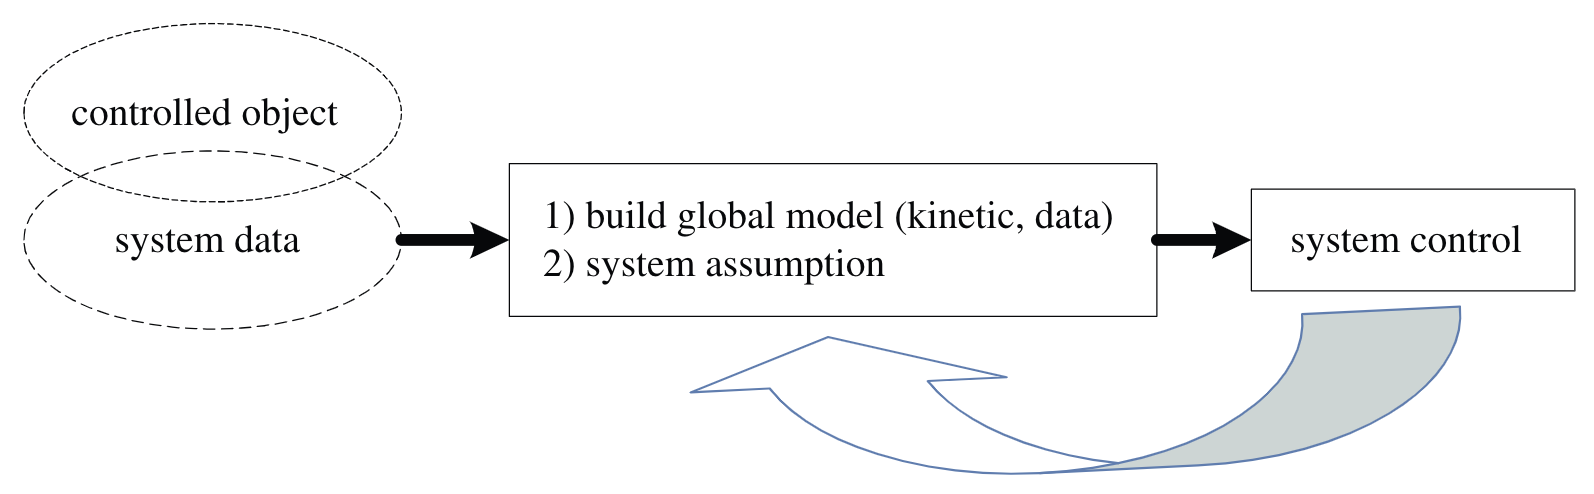
\includegraphics[width=.75\textwidth]{Screenshots for paper/1.png}}
\caption{Common structure of the Model Based Control \cite{hou2013model}}
\label{fig:mbcsctruct}
\end{figure}

\subsection{Data Driven Control}

Opposed to the Model Based Control, Data Driven control is becoming more popular. \cite{hou2013model} suggest the following definition for Data-Driven control: "Data-driven control includes all control theories and methods in which the controller is designed by directly using on-line or off-line I/O data of the controlled system or knowledge from the data processing but not any explicit information from mathematical model of the controlled process, and whose stability, convergence, and robustness can be guaranteed by rigorous mathematical analysis under certain reasonable assumptions". Data-Driven control for various purposes is becoming the superior method in systems where the model is not available or is changing over the course of life cycle, i.e. adaptability is necessary. This implies that motors and other motile systems are the ones which need Data-Driven control the most. Data-Driven controller design method allows to bypass the tedious system identification step. However, as every machine learning problem, it requires big amounts of data. This becomes less of a problem year by year, as every industry, be it information technology or metallurgy, is becoming more and more digitized and thus produces vast amounts of data. This data has a vast potential of improving the current processes if processed correctly. The data gathered from the system behaviour is used to identify the controller. In this paper, we investigate the application of data-driven control to the control of DC motor drives and experiment with data-driven controller estimation using reinforcement learning.

\subsection{DC motors}
DC motors are an inseparable part of modern motile systems in engineering and robotic system control. They are efficient and are able to be controlled in various ways. 




\chapter{\label{chapter2} Related Work}


The article written by Naung et al. \cite{naung2018a} is closely related to our work by the research aims and methods. Authors present Data-Driven Control used for system parameters identification, an approach that we are planning to use. The main goal of the paper is to perform system identification utilizing the data driven system control of the DC motor, with ultimate generation of the transfer function suitable for robust control of the plant. For this purpose, authors use MATLAB to create the Simulink model of the DC motor (Figure \ref{fig:dcsimulink}) and calculate the proportional-integral-differential (PID) controller according to the obtained models.

\begin{figure} [h!]
\centerline{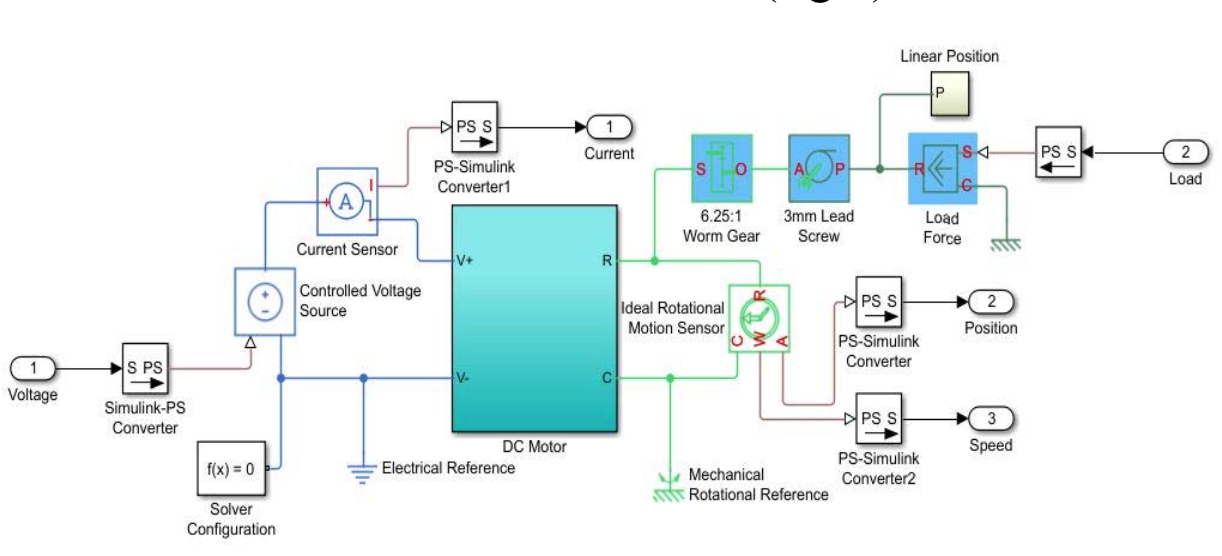
\includegraphics[width=.75\textwidth]{Screenshots for related work/1.png}}
\caption{Simulink diagram of simscape physical plant DC motor \cite{naung2018a}.}
\label{fig:dcsimulink}
\end{figure}

Authors compare the performance of the nonlinear autoregressive exogenous inputs (NARX) artificial neural network and nonlinear black-box model structures, summarized in Figure \ref{fig:pidcomparison}. They conclude that the proposed control method performs with acceptable accuracy and is utilizable with more complex dynamic systems. 

\begin{figure}
\centerline{
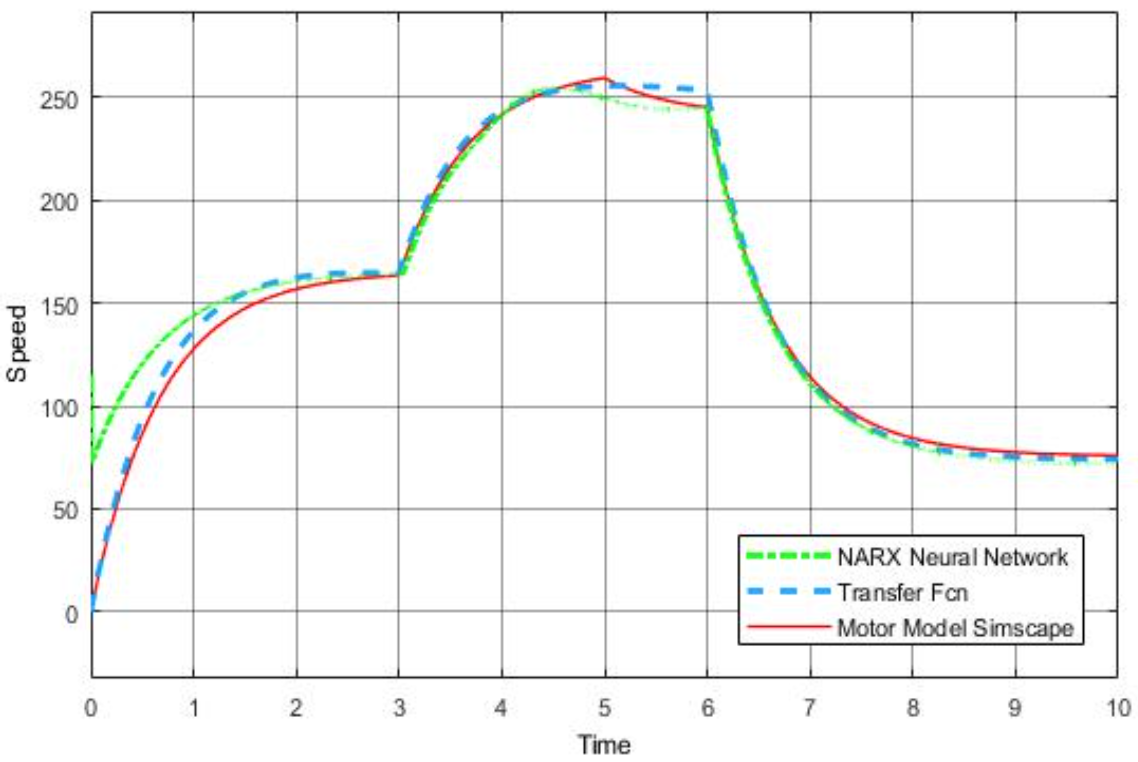
\includegraphics[width=.47\textwidth]{Screenshots for related work/2.png}\hfill
\label{NARX ANN}
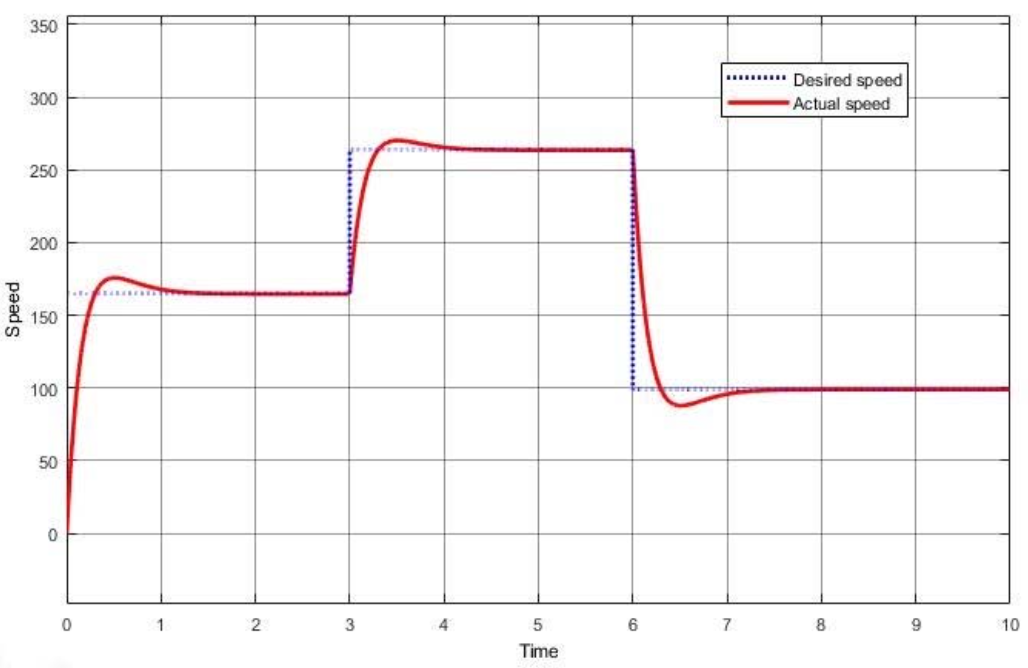
\includegraphics[width=.49\textwidth]{Screenshots for related work/3.png}
\label{PID controller}
}
\caption{Results of the speed response of the DC motor using NARX Neural Network and PID controller \cite{naung2018a}.}
\label{fig:pidcomparison}
\end{figure}

Coulson, Lygeros, and Dorfler introduce novel data-enabled predictive
control (DeePC) algorithm \cite{coulson2019data}, that utilizes real-time feedback of the system, and is able to drive the system along a desired trajectory with given system constraints. The DeePC  algorithm  was  applied  to unknown linear time-invariant (LTI)  system  and was compared to classical Model  Predictive  Control (MPC) algorithm. Authors state that the DeePC was created with thinking from a behavioural systems theory perspective. The algorithm description is provided in both mathematical proof form and a pseudo-code description of the algorithm steps. As an example of sophisticated nonlinear application of the DeePC, a case, a regularized version of the algorithm was simulated on  stochastic nonlinear quadcopter dynamics, illustrating its capabilities beyond deterministic LTI systems - figure \ref{fig:quadsim}.

\begin{figure} [h!]
\centerline{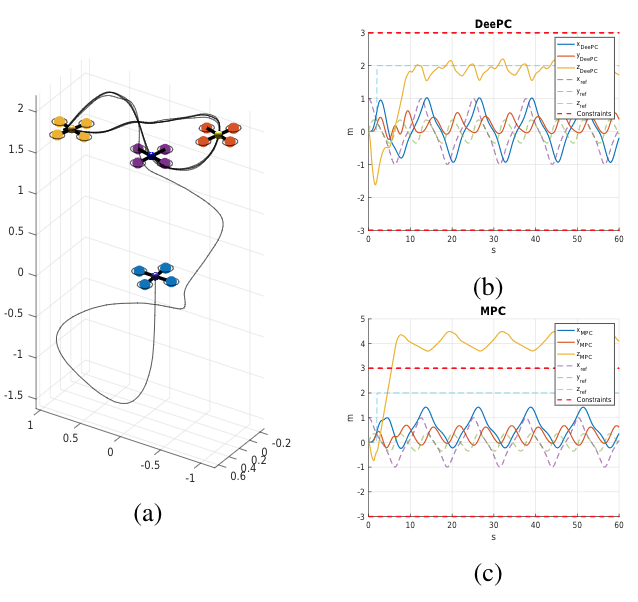
\includegraphics[width=.75\textwidth]{Screenshots for related work/5.png}}
\caption{Figure (a): three dimensional plot of the trajectory of the quadcopter at different instances of time controlled with DeePC.  Figure  (b)  and  (c):  trajectories  of  the  spatial  coordinates  when  controlled  by  DeePC  and  MPC,  respectively. The horizontal red dashed lines represent constraints.
\cite{coulson2019data}}
\label{fig:quadsim}
\end{figure}

A recent work by Carlet et al. \cite{carlet2020data} utilizes the aforementioned DeePC algorithm in a setup with motors. This is an important article for our project, as it explores predictive current control for permanent  magnet synchronous motor drives - a topic closely related to ours. Authors utilize two  of  the  most  popular data-driven   algorithms - the   Subspace Predictive  Control  algorithm  and  the  Data-Enabled  Predictive Control  algorithm. Current  controller  design  procedure for both methods is discussed and presented in detail. Simulation results are reported to be comparably robust and with strong correlation for both of the unconstrained  and  constrained  versions  of  the  data  driven  methods, as it could be seen in figure \ref{fig:controllercomp}.

\begin{figure} [h!]
\centerline{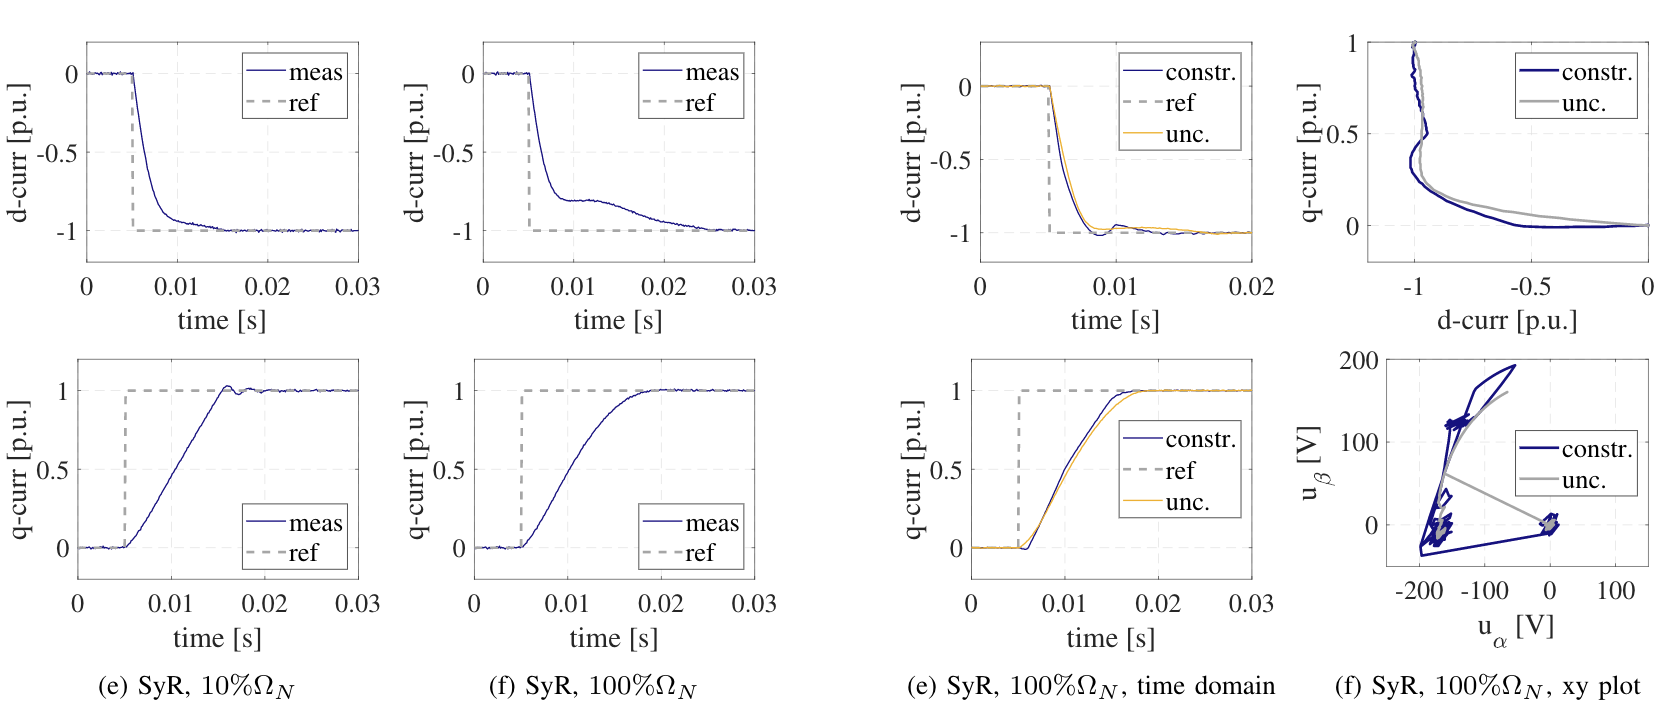
\includegraphics[width=.95\textwidth]{Screenshots for related work/4.png}}
\caption{Step response of SPC data-driven current controllers
\cite{carlet2020data}}
\label{fig:controllercomp}
\end{figure}

Hou and Wang created a canonical survey paper in the field in 2013 \cite{hou2013model}. Almost every other related work cites this paper, as it contains fundamental definitions for the Data driven control and its applications. The paper begins with a brief description and comparison of Model based control theory and Data driven control theory. Motivation for the data based control is stated as well. Further, they state the focus of data-driven control theory in terms of objects that could be controlled with the use of it. For the rest of the survey paper authors explore the recent advances in DDC and discuss the perspectives of future related work. They conclude with categorization of different available Data-driven techniques according to required usage. However, the survey's drawback is that most of the methods are currently outdated, as this is a fast evolving field. The general introductory information provided by the authors is nevertheless valuable.



Next article by Hanke, Wallscheid and Bocker \cite{hanke2019continuous}  introduces Permanent Magnet Synchronous Motor ripple avoidance using DDC. It also compares three types of linear controllers and the input/output data.

\begin{figure} [h!]
\centerline{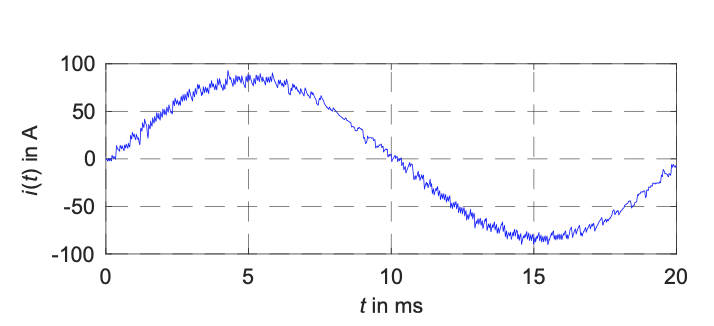
\includegraphics[width=.75\textwidth]{Screenshots for related work/Asset p1/Asset p1p1.png}}
\caption{CCS-MPC at 60A
\cite{hanke2019continuous}}
\label{fig:p1p1}
\end{figure}

\begin{figure} [h!]
\centerline{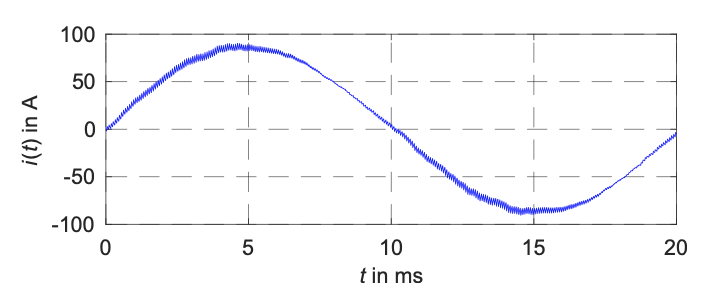
\includegraphics[width=.75\textwidth]{Screenshots for related work/Asset p1/Asset p1p2.png}}
\caption{FOC at 60A
\cite{hanke2019continuous}}
\label{fig:p1p2}
\end{figure}

\begin{figure} [h!]
\centerline{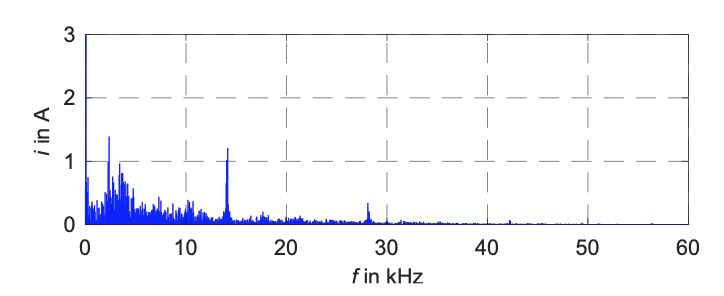
\includegraphics[width=.75\textwidth]{Screenshots for related work/Asset p1/Asset p1p3.png}}
\caption{CCS-MPC at 60A
\cite{hanke2019continuous}}
\label{fig:p1p3}
\end{figure}

\begin{figure} [h!]
\centerline{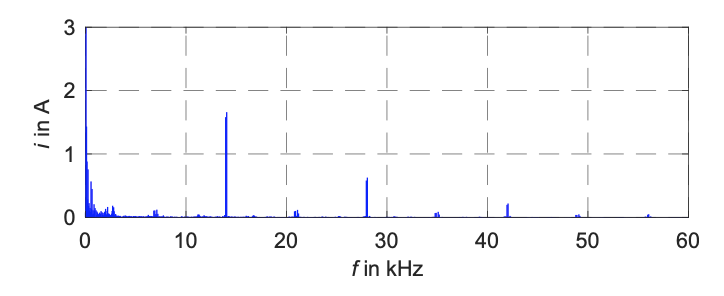
\includegraphics[width=.75\textwidth]{Screenshots for related work/Asset p1/Asset p1p4.png}}
\caption{FOC at 60A
\cite{hanke2019continuous}}
\label{fig:p1p4}
\end{figure}

We can clearly see that total harmonic distortion of the FOC system is smaller and that CCS-MPC only better at those special harmonics of the three phase system. 

Article \cite{de2019a} discusses the important attributes for systems with data-driven control: Stabilization, Optimality, and Robustness. Authors argue that it is possible to create a linear approximation of a non linear closed loop system using only data-dependant linear matrix equations. 

Article \cite{rosolia2018a} explores the ability of the data-driven system to adapt and thus improve its performance in case of changes of parameters. The author argues that it is possible to have a learning model that could be started without correct initial state and even learn from data without diverging back from better state, which is backed by simulation. Each discreet step of the controller is used as an iteration for the learning algorithm. Model Predictive Control (MPC) was chosen as a back-bone for the closed loop control and re-applied as MPC for Batch processes (iterations) and then replaced by LQR as LMCPC. 

\begin{figure} [h!]
\centerline{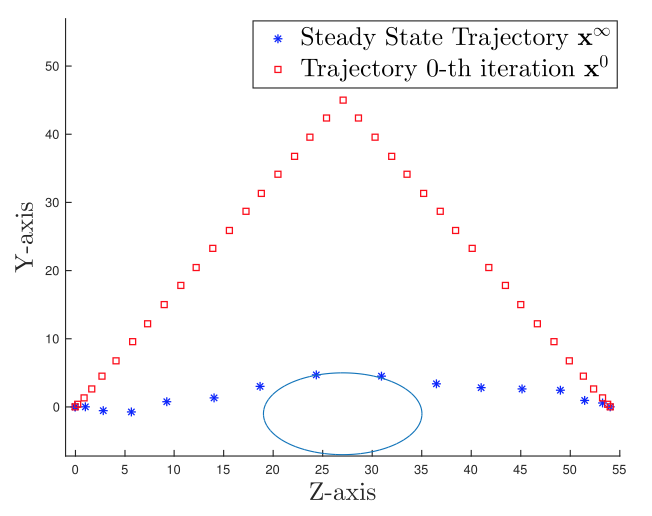
\includegraphics[width=.75\textwidth]{Screenshots for related work/Asset p2/Asset p2p1.png}}
\caption{SS positions over ZY plane
\cite{rosolia2018a}}
\label{fig:p2p1}
\end{figure}


Article \cite{bu2018a} analyzes the behavior of data-driven control in the extreme case of output saturation. This paper also uses a linear system approximation approach with dynamic linearization, but also applies assumption that the system has an output saturation. This does increase the tracking performance but decreases the resting time of the closed loop system. 

Article \cite{pravallika2021a} is an official MATLAB tutorial to DDC, which we follow with our designed controller simulation in the beginning of our project.

A recent article \cite{Berberich_2020} overviews a problem of state-feedback controllers for discrete-time linear time-invariant systems, based directly on measured data. This paper presents the robust methods for data-driven control in which the stable closed-loop performance is guaranteed even in presence of noise in data. The design of state-feedback controllers is based on the parametrization technique analyzed in \cite{de2019a}, particularly the application of robust control techniques to the parametrization, which results in stable performance of the closed loop control with noisy inputs.

In the paper \cite{piga2017direct} a data-driven approach is used to design a hierarchical controller which includes the inner and outer controllers to enhance the overall performance of the inner controller. The evaluation of the effectiveness of this type of method is done by means of simulation and practical experiments. Basically this paper proposes the implementation of the outer Model Predictive controller used for improving the performance of an inner closed loop controller. In such a way it is not only improves the overall performance of the system, but also takes care of constraints imposed on inputs and outputs. Figure \ref{fig:hierarchicalcontroller} shows the resultant hierarchical controller, in which it can be seen that the outer Model Predictive controller tracks the input and output variables and operates on the reference signal applied to the inner loop in order to satisfy the constraints imposed on inputs and outputs of an overall system as well as improve on the system performance. To test the results the simulation of a servo positioning system in dc motor was used. The inner loop controller design resulted in the following performance shown in figure \ref{fig:innerloopcontroller}. However because of the lower degrees of freedom of the controller the controller could not obtain the faster dynamics and thus resulted in slow dynamics with the rise time of about 4 s. Adding the model predictive controller resulted in much better performance as shown in figure \ref{fig:controllerwithMPC} below. The rise time resulted in 1.3 s, which is about 3 times as much faster as the previous result. 

\begin{figure} [h!]
\centerline{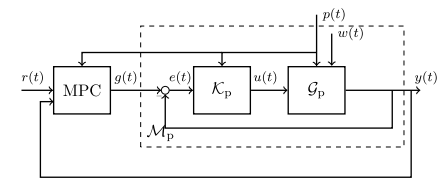
\includegraphics[width=.75\textwidth]{Screenshots for related work/constraint_data_driven_control_screenshot1.png}}
\caption{Proposed hierarchical control architecture
\cite{piga2017direct}}
\label{fig:hierarchicalcontroller}
\end{figure}

\begin{figure} [h!]
\centerline{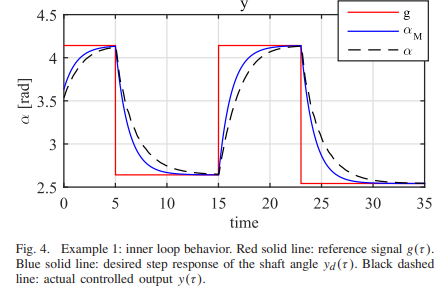
\includegraphics[width=.75\textwidth]{Screenshots for related work/constraint_data_driven_control_screenshot2_innerloop.png}}
\caption{Inner loop behaviour
\cite{piga2017direct}}
\label{fig:innerloopcontroller}
\end{figure}

\begin{figure} [h!]
\centerline{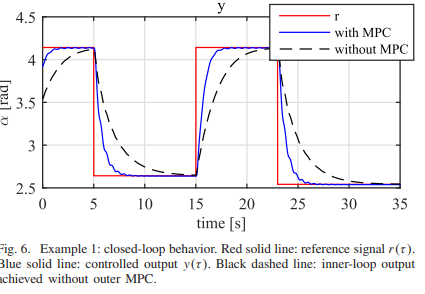
\includegraphics[width=.75\textwidth]{Screenshots for related work/constraint_data_driven_control_screenshot2_usingMPC.png}}
\caption{Closed loop behaviour with added MPC
\cite{piga2017direct}}
\label{fig:controllerwithMPC}
\end{figure}

A PhD thesis \cite{kergus} explores a Data-driven model reference control in the frequency-domain. 

An article \cite{CAMPESTRINI20172628} deals with Data-Driven (DD) control design in a Model Reference (MR) framework. 

Article \cite{vuillemin2019hybrid} shows a discrete-time control-law from frequency-data of a continuous-time plant so that their hybrid interconnection matches a given continuous-time reference model up to the Nyquist
frequency. 

Article \cite{Waarde2020} Data Informativity: A New Perspective on Data-Driven Analysis and Control

\chapter{Design approaches and Methods}

po idee Arduino i dSpace eto uzhe Implementation, ne? Suda nuzno pro simulation :D

\section{MATLAB simulation}
\subsection{Motor model identification}
\subsubsection{data gathering}

\begin{figure} [h!]
\centerline{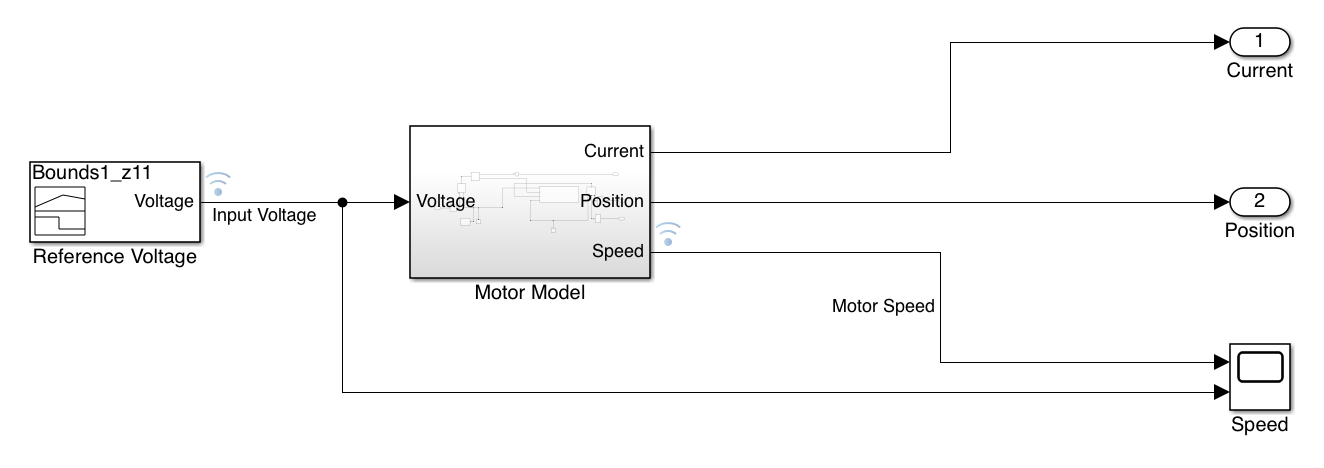
\includegraphics[width=.75\textwidth]{Screenshots for paper/matlab models/data aq model.png}}
\caption{MATLAB model to workspace data acquisition Simulink model}
\label{fig:MATLABmodelAT1}
\end{figure}

\begin{figure} [h!]
\centerline{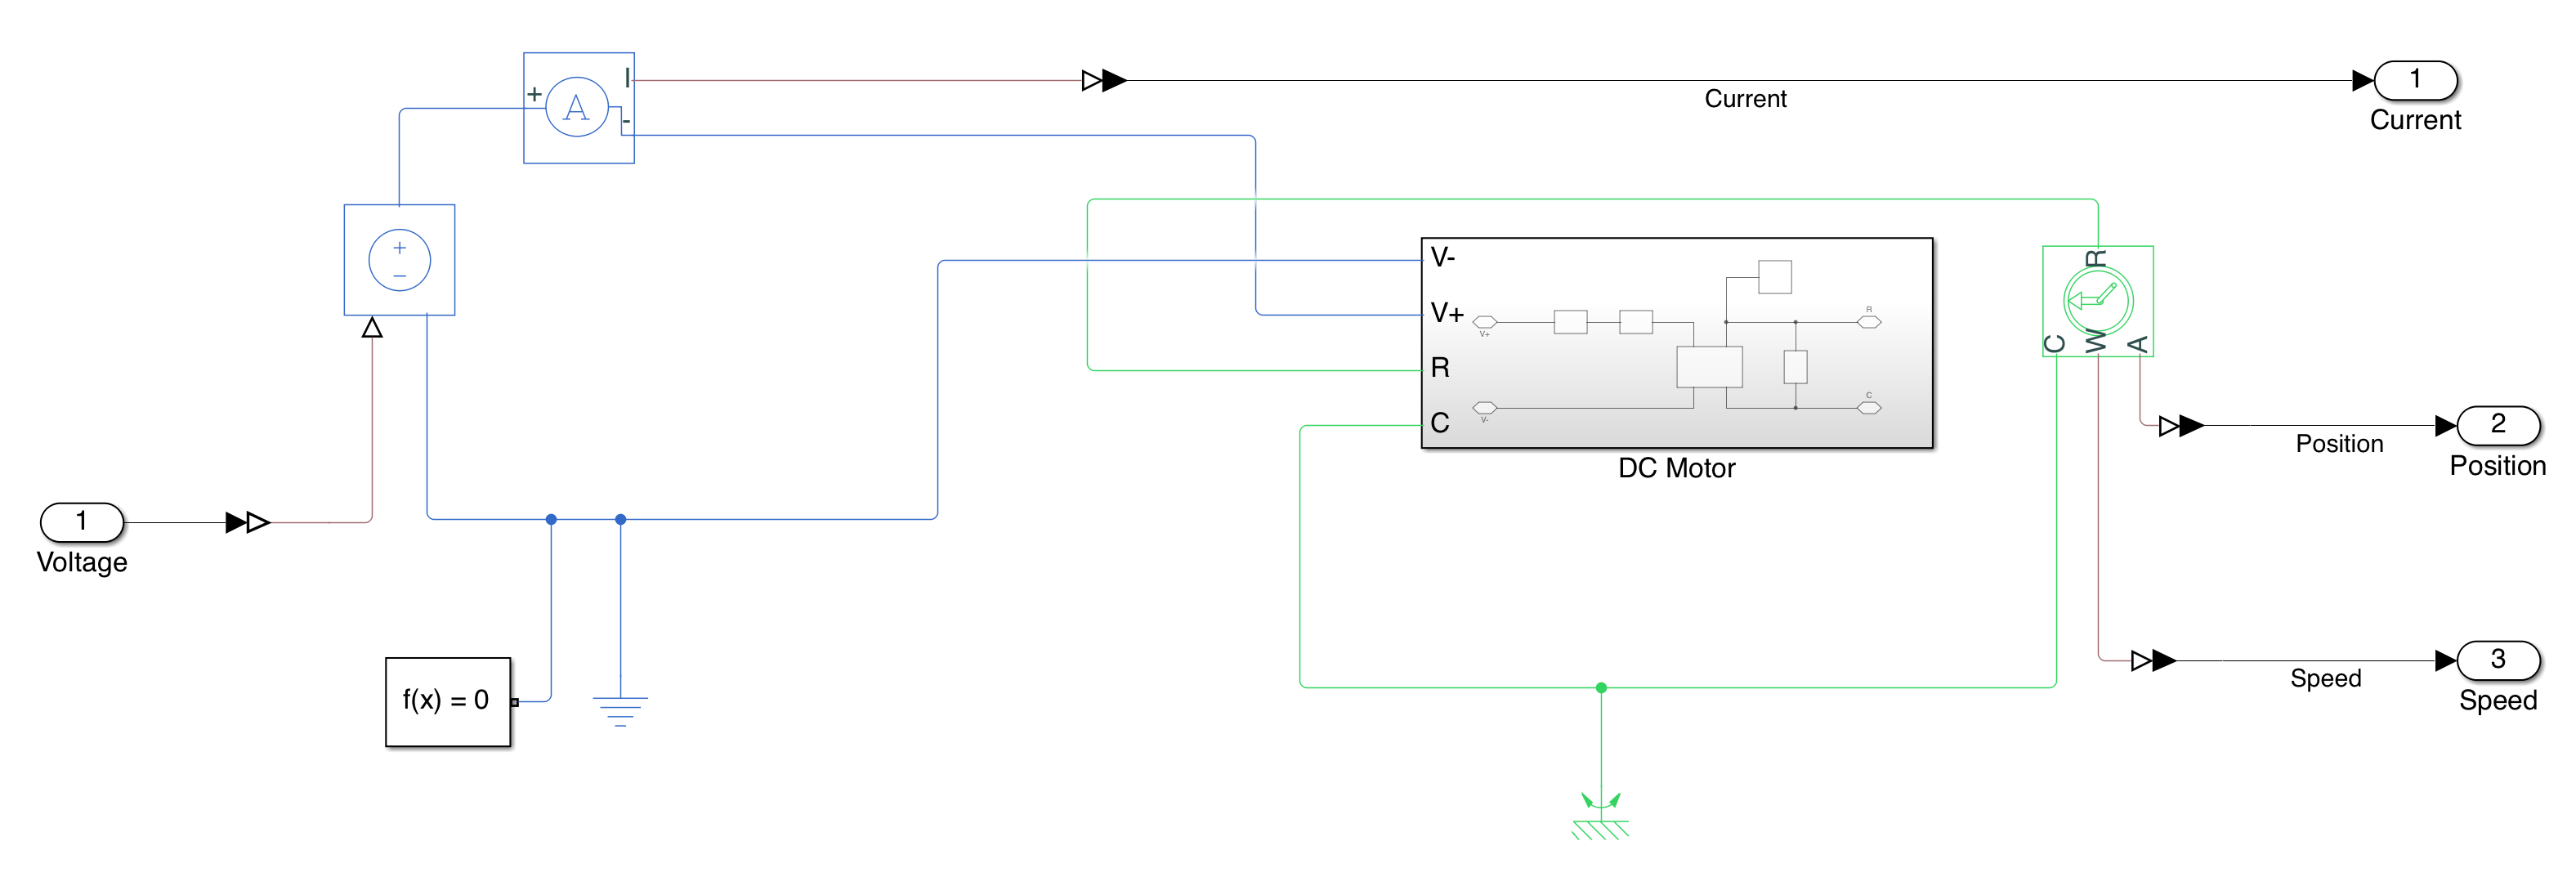
\includegraphics[width=.75\textwidth]{Screenshots for paper/matlab models/Motor Model.png}}
\caption{MATLAB Simulink Motor Model}
\label{fig:MatlabMotorModel}
\end{figure}

\begin{figure} [h!]
\centerline{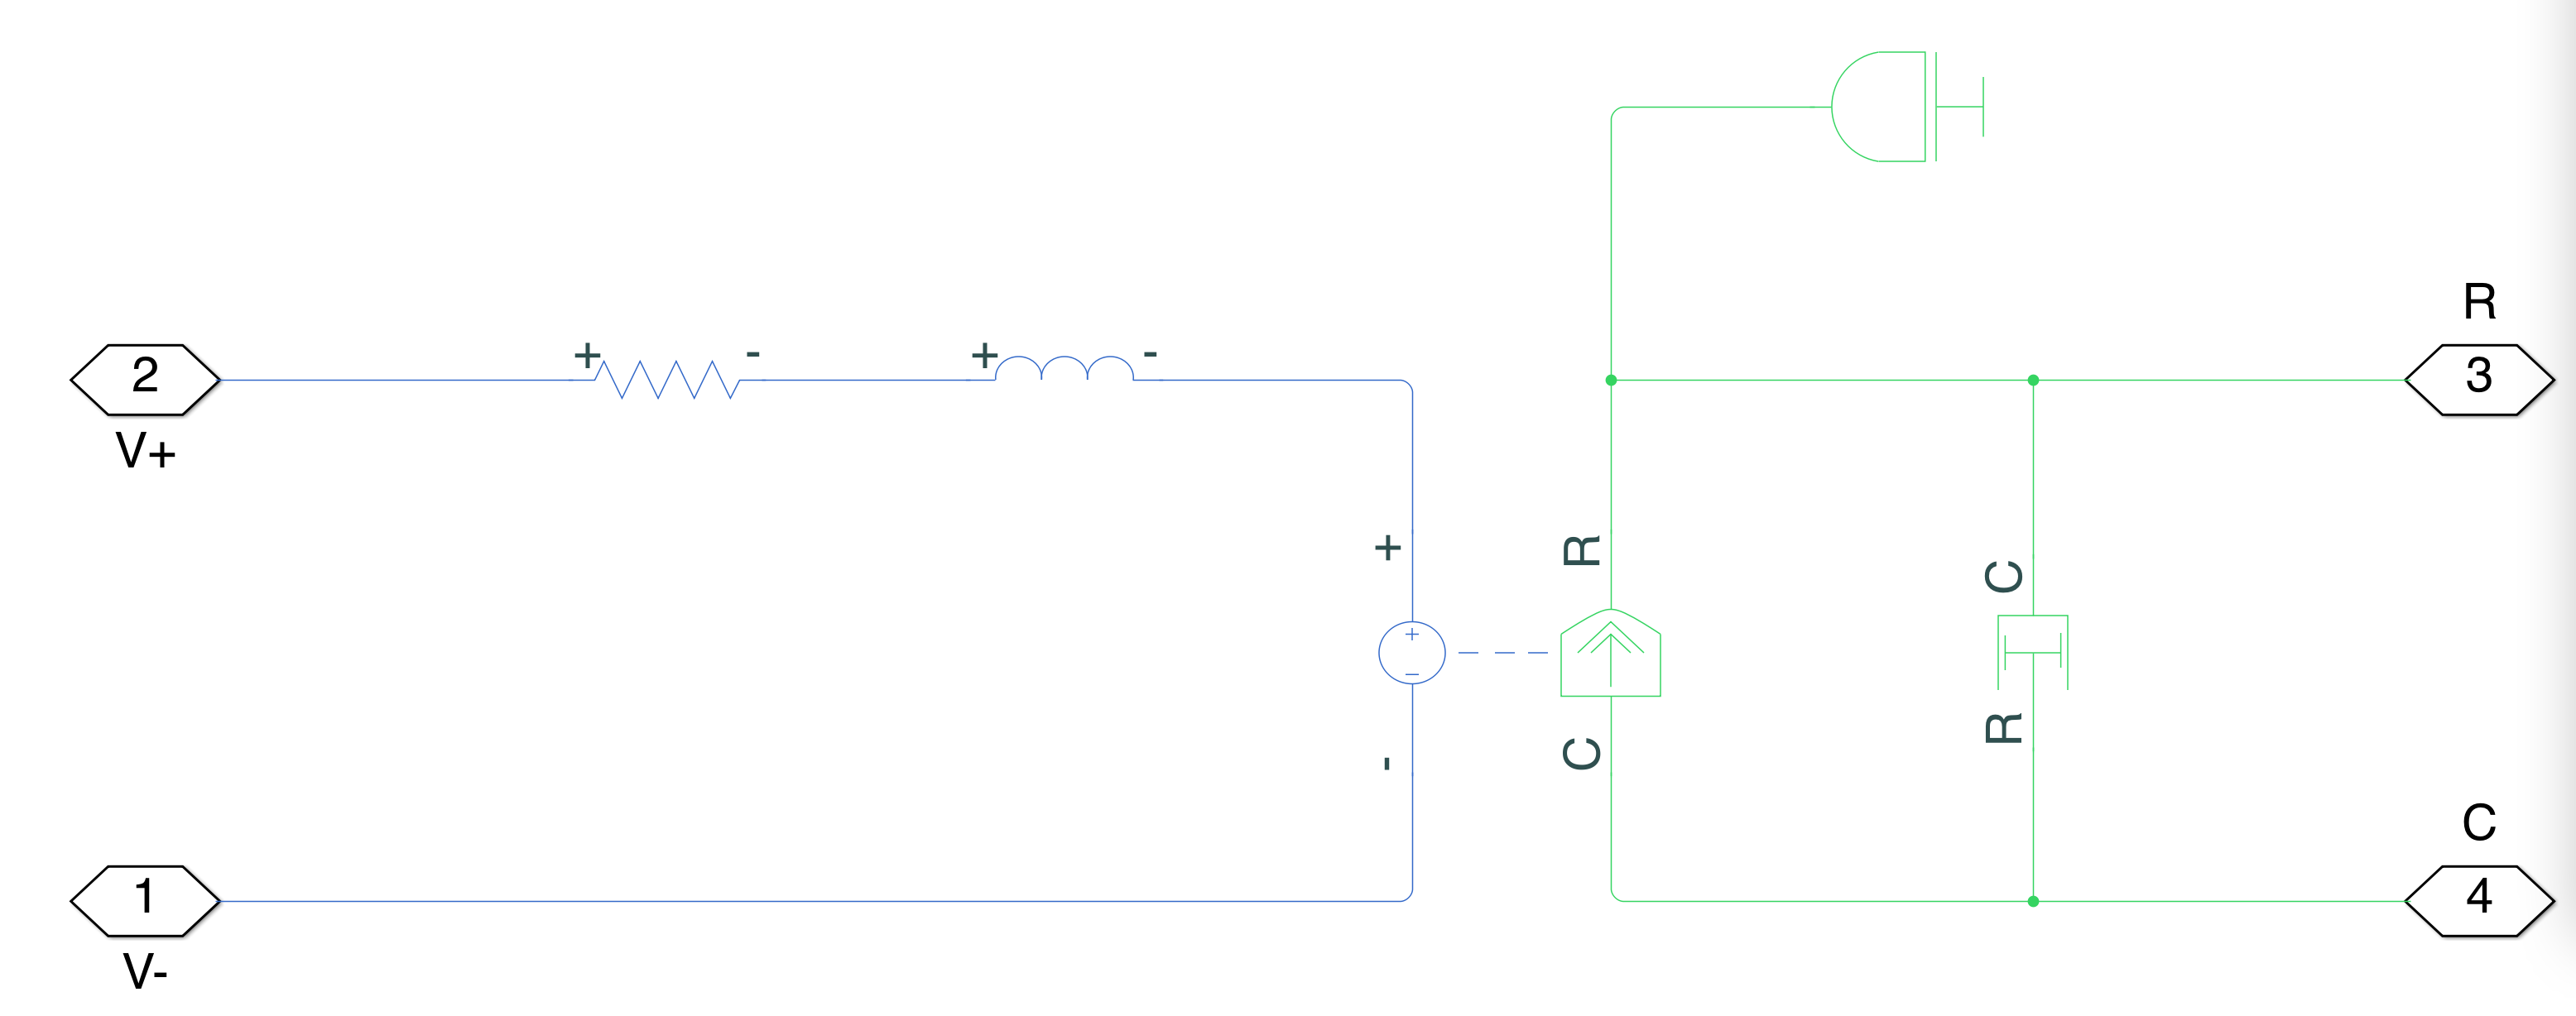
\includegraphics[width=.75\textwidth]{Screenshots for paper/matlab models/DC Motor.png}}
\caption{MATLAB Simulink DC Motor isolated part}
\label{fig:MatlabMotorDCpart}
\end{figure}

\subsubsection{Data pre-processing}
tut napishi kak tu delal z1 z2 z4 z7 z9 -> single datastream

\subsubsection{Model identification and fitting}

\subsubsection{testing with PID Controller}

\chapter{Implementation}

\section{Arduino}

\begin{figure} [h!]
\centerline{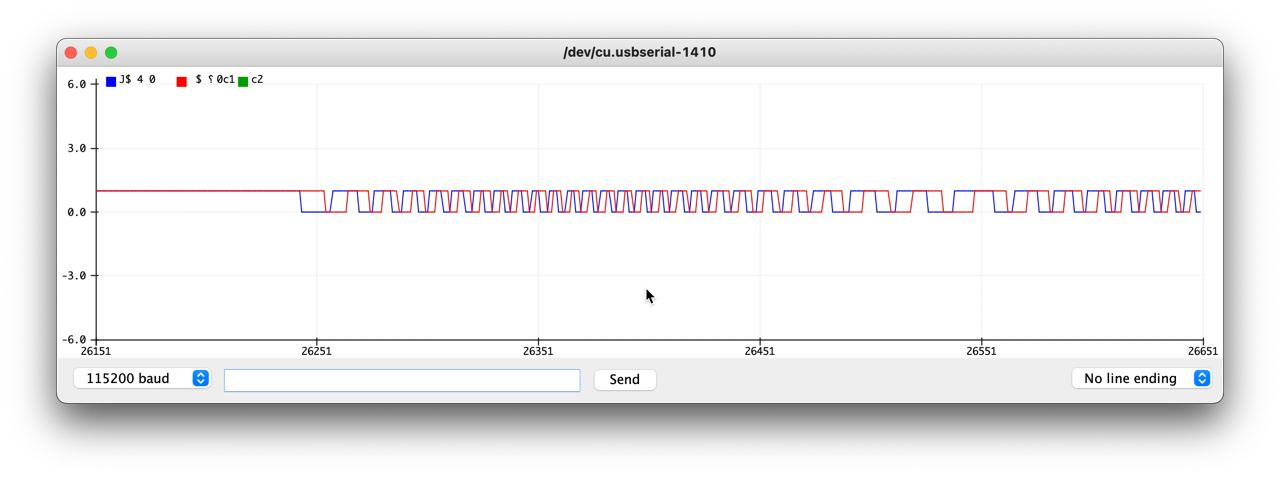
\includegraphics[width=.75\textwidth]{Screenshots for paper/arduino/encoder signal.jpeg}}
\caption{Arduino plot for encoder signal}
\label{fig:arduinoEncoder}
\end{figure}

Arduino IDE is a software environment that creates near native machine code with included Arduino.h header. Figure \ref{fig:arduinoEncoder} shows the incoder signal plotted using Arduino.h's digital read and Serial plot libraries. The signal is produced by rotating rotor with encoder by hand. This might be important because even thought signal looks great, it is plotted on low angular velocity.

\begin{figure} [h!]
\centerline{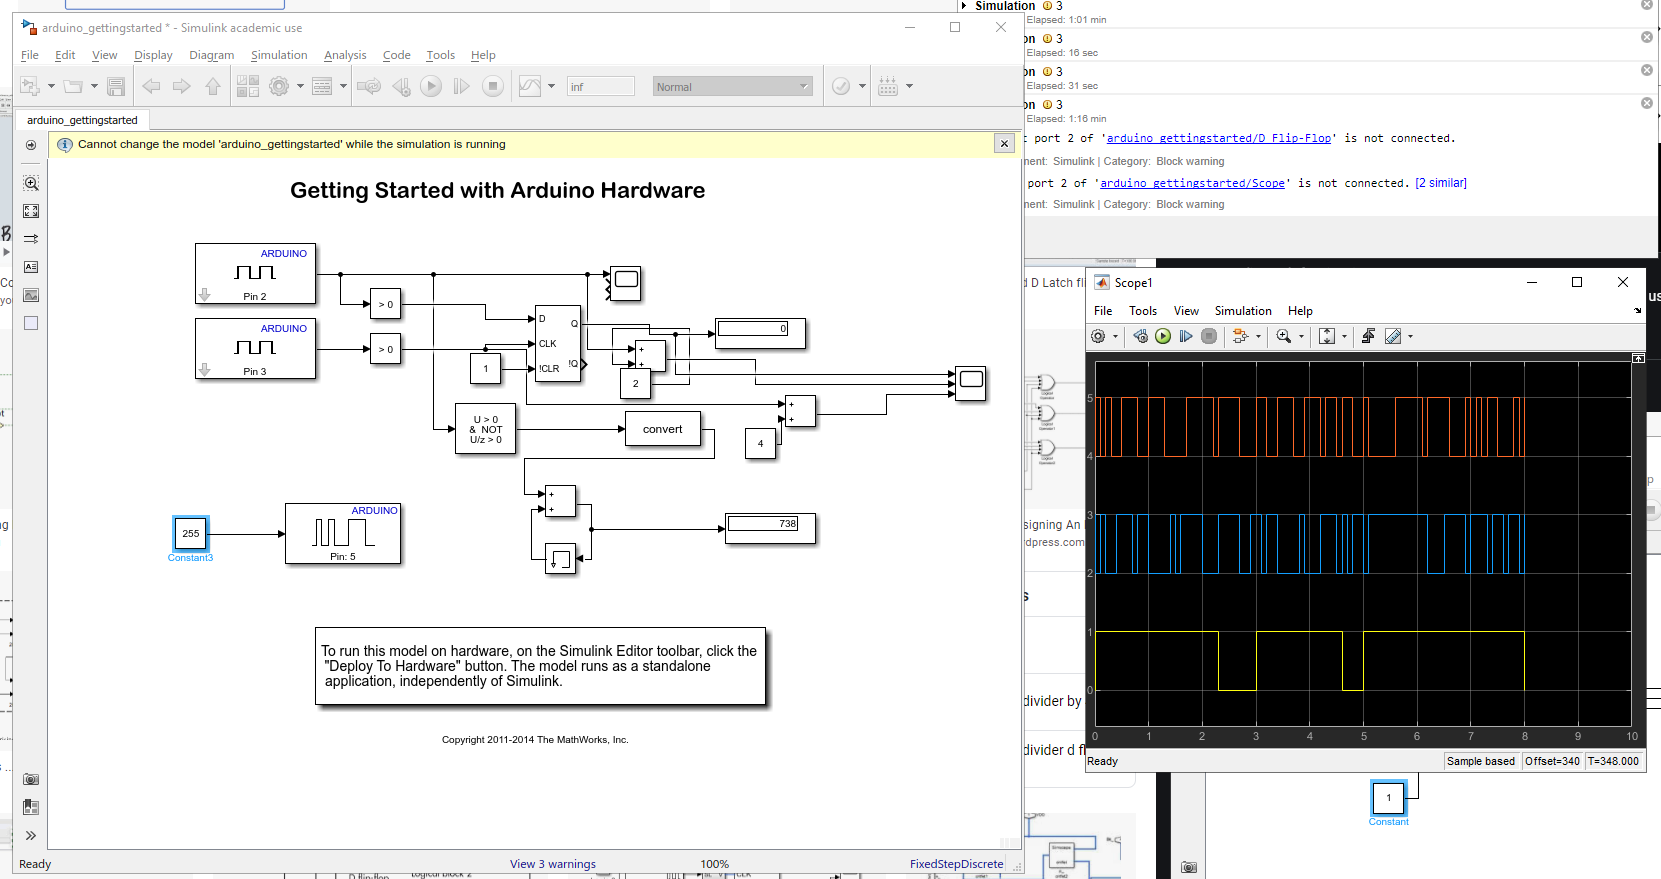
\includegraphics[width=.75\textwidth]{Screenshots for paper/arduino/Model encoder arduin MATLAB.PNG}}
\caption{MATLAB Simulink Arduino model}
\label{fig:arduinoSimulink}
\end{figure}

After checking encoder signal we assembled a MATLAB Simulink \ref{fig:arduinoSimulink} model to be able to read encoder's speed and direction. This time rotor was driven by applied voltage on the motor. This way we got stable uniform encoder signal to check the encoder velocity units and direction. We were partially successful. Quick observation shows that even though the motor had constant velocity with no load or oscillations on direction the model showed chaotic alternation in motor direction. After analysing the recorded signal we come to the conclusion that model with Arduino could not keep up with the signal and the samples resulted in aliasing. This was further proven when we tried to increase the sample frequency of the Arduino simulink model. There is a possibility that there is some additional sample rate related parameters of the model that could solve problem with aliasing, but we did not find it and came to a conclusion that Arduino's MATLAB Simulink implementation is just simply not fast enough. There could be made a walk-around by coding the Arduino with its native Arduino IDE to minimize the overhead and set up custom bare minimum communication method over virtual com port UART.

\section{dSpace}

After somewhat successful attempt of data gathering with 
\begin{figure} [h!]
\centerline{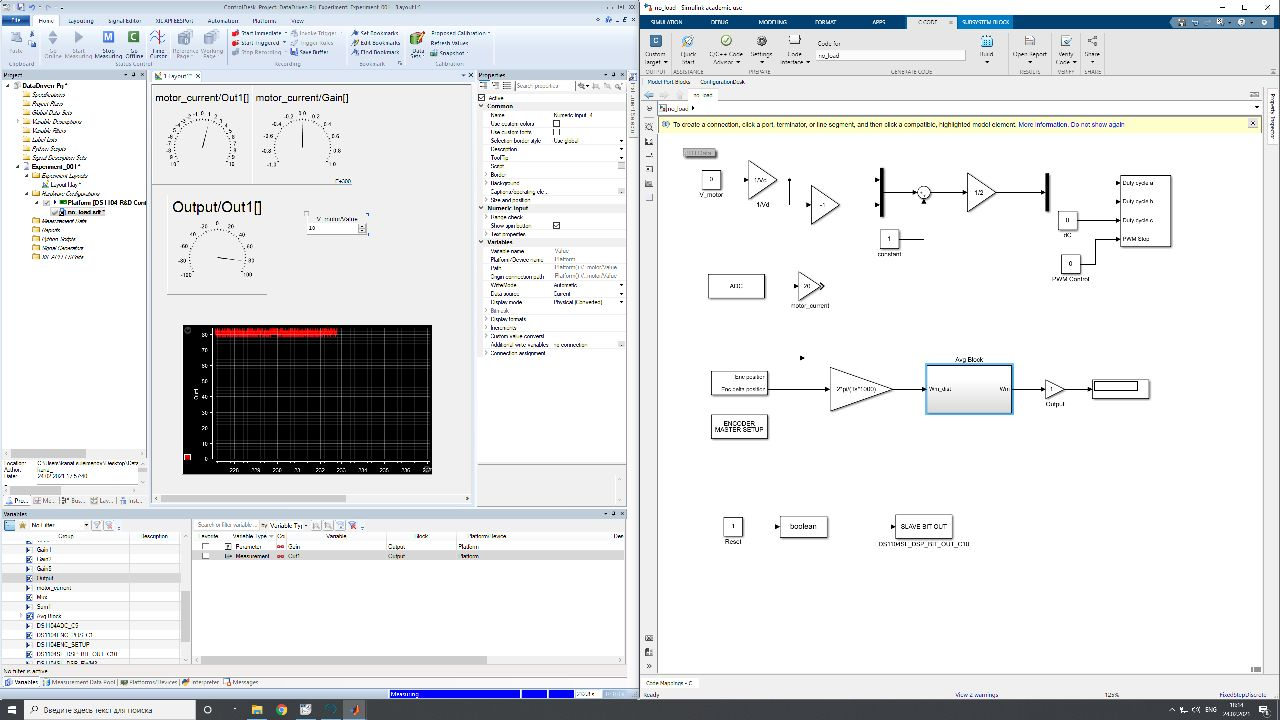
\includegraphics[width=.75\textwidth]{Screenshots for paper/dSpace/photo_2021-03-09 11.37.29.jpeg}}
\caption{dSpace workspace for data gathering}
\label{fig:dSpaceEx1}
\end{figure}



\chapter{Results}

\chapter{Conclusion and Future work}




%%%% ADD YOUR BIBLIOGRAPHY HERE
\newpage
\bibliographystyle{ieeetr}
\bibliography{bibliography} 

\label{endpage}


\end{document}

\end{article}
